\subsection*{Problema 19}
\textbf{Enunciado:} Calcular la integral:
\begin{equation*}
\int \frac{3x^2 + 2x - 2}{x^3 - 1} \, dx
\end{equation*}

\textbf{Solución:} 
Utilizamos la descomposición en fracciones parciales. El denominador se factoriza como:
\begin{equation*}
x^3 - 1 = (x - 1)(x^2 + x + 1)
\end{equation*}

Planteamos la forma de las fracciones parciales:
\begin{multline*}
\frac{3x^2 + 2x - 2}{x^3 - 1} = \frac{A}{x - 1} \\
+ \frac{Bx + C}{x^2 + x + 1}
\end{multline*}

Multiplicando por el denominador común:
\begin{multline*}
3x^2 + 2x - 2 = A(x^2 + x + 1) \\
+ (Bx + C)(x - 1)
\end{multline*}

Evaluamos en $x = 1$ para hallar $A$:
\begin{equation*}
3(1)^2 + 2(1) - 2 = A(1^2 + 1 + 1)
\end{equation*}
\begin{equation*}
3 = 3A \implies A = 1
\end{equation*}

Expandimos y agrupamos términos según las potencias de $x$:
\begin{multline*}
3x^2 + 2x - 2 = (A + B)x^2 \\
+ (A - B + C)x + (A - C)
\end{multline*}

Igualando coeficientes:
\begin{align*}
A + B &= 3 \\
A - B + C &= 2 \\
A - C &= -2
\end{align*}

Como $A = 1$, obtenemos $B = 2$ y $C = 3$. La integral se reescribe como:
\begin{equation*}
\int \left( \frac{1}{x - 1} + \frac{2x + 3}{x^2 + x + 1} \right) dx
\end{equation*}

Para el segundo término, ajustamos el numerador para que sea la derivada del denominador ($2x + 1$):
\begin{multline*}
\int \frac{2x + 3}{x^2 + x + 1} \, dx = \int \frac{2x + 1}{x^2 + x + 1} \, dx \\
+ \int \frac{2}{x^2 + x + 1} \, dx
\end{multline*}

Completando el cuadrado en el último término:
\begin{equation*}
x^2 + x + 1 = \left(x + \frac{1}{2}\right)^2 + \frac{3}{4}
\end{equation*}

Integramos cada parte:
\begin{multline*}
\int \frac{3x^2 + 2x - 2}{x^3 - 1} \, dx = \ln|x - 1| \\
+ \ln|x^2 + x + 1| \\
+ \frac{2}{\frac{\sqrt{3}}{2}} \arctan\left(\frac{x + \frac{1}{2}}{\frac{\sqrt{3}}{2}}\right) + C
\end{multline*}

Simplificando el resultado final:
\begin{multline*}
= \ln|x^3 - 1| \\
+ \frac{4}{\sqrt{3}} \arctan\left(\frac{2x + 1}{\sqrt{3}}\right) + C
\end{multline*}

\begin{figure}[H]
	\centering
	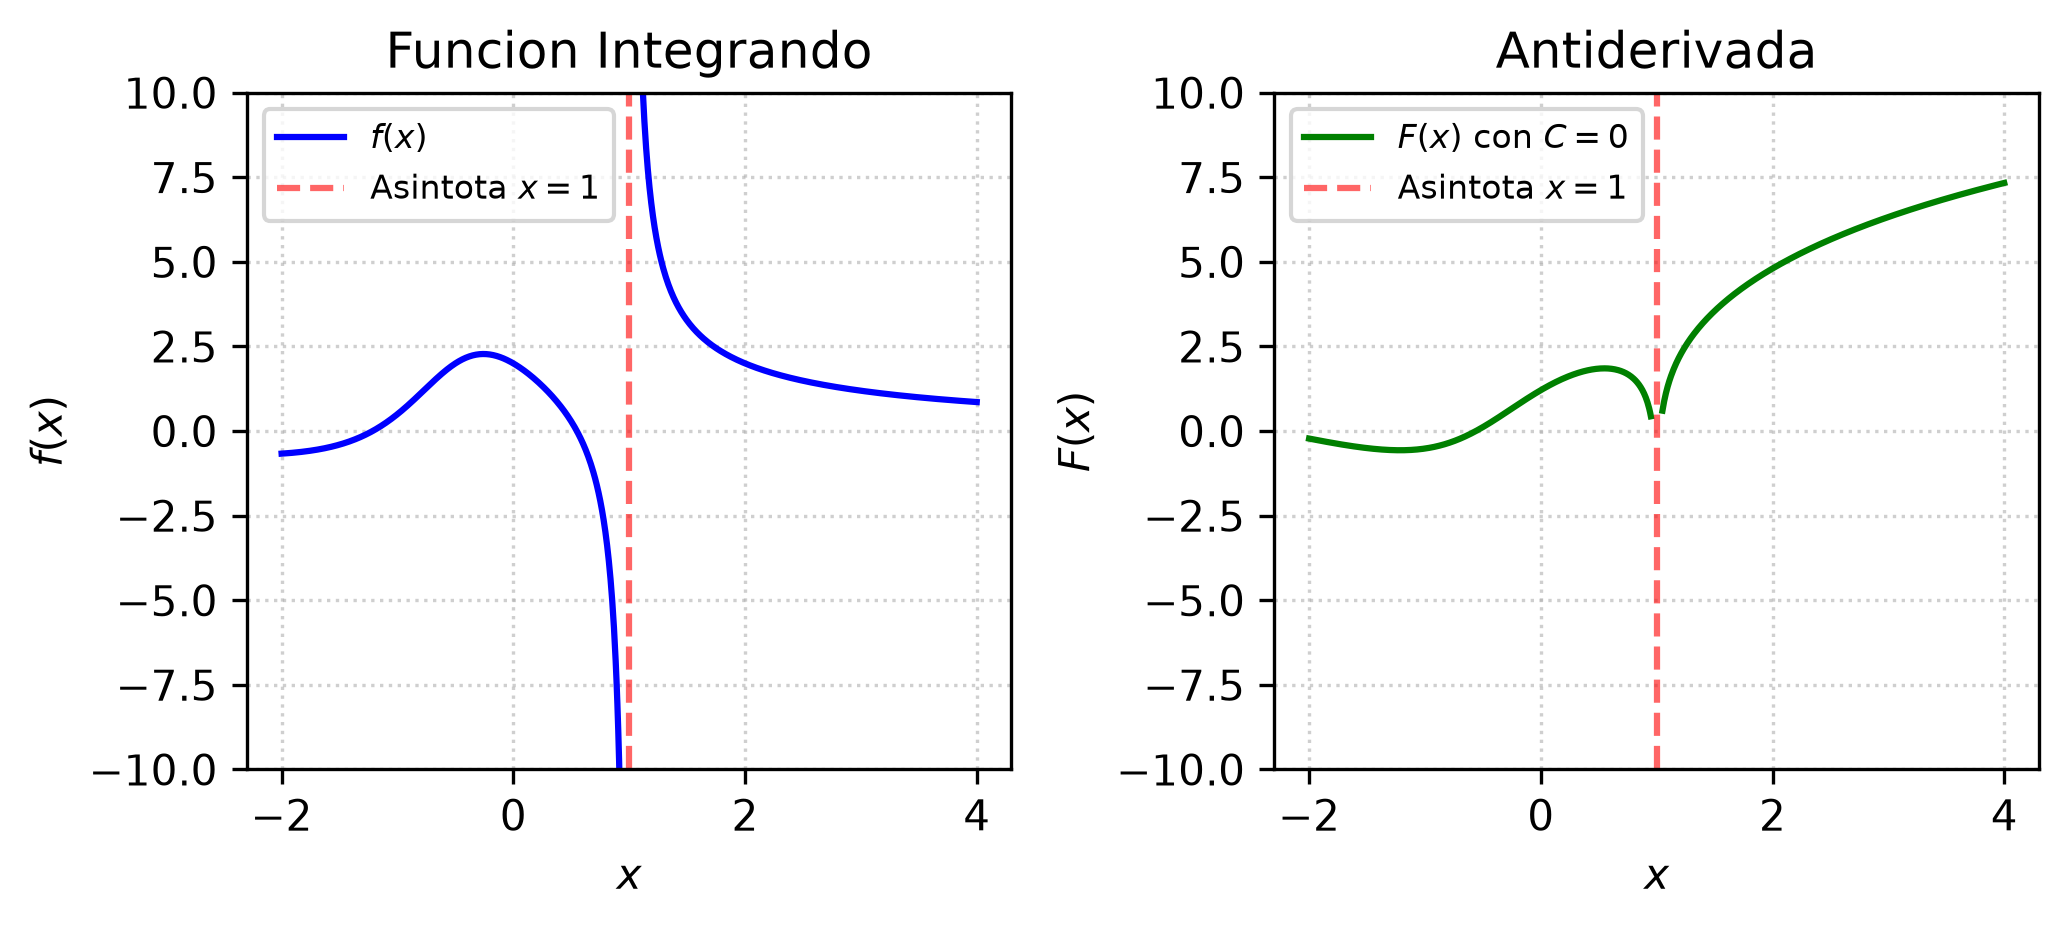
\includegraphics[width=\columnwidth]{semana_03/graficas/SEM03_P19_grafica.png}
	\caption{Representación gráfica de $f(x)$ y su antiderivada $F(x)$ evaluada para la constante de integración $C = 0$ (Problema 19).}
	\label{fig:problema19}
\end{figure}
